% !TeX root = ../../main.tex
% Add the above to each chapter to make compiling the PDF easier in some editors.

\chapter{Benchmark Methods}\label{ord:ch3}

In this chapter the interactive methods used in the benchmark study are introduced.
Their technical functionality is explained in detail, while the motivation behind their selection is discussed in Section \ref{ord:ch4:sec2}.

The following methods all perform in the same setup: An image, that contains one or multiple objects, is shown to the user and the user's task is to create separate masks for the objects in the image.
To segment multiple objects in one image, the method has to be applied for each object separately.
The images are usually colored and contain the three color channels \gls{rgb}.
%TODO what about gray scale images
%TODO class-agnostic image segmentation

% !TeX root = ../../main.tex
% Add the above to each chapter to make compiling the PDF easier in some editors.

\section{Polygon Drawing}\label{ord:ch3:sec1}

In contrast to previously introduced methods, this polygon drawing proceeds manual.
By manually setting points on the object in the image a polygon is created.
From three points a polygon is spanned, where each point functions as a node.
% Each point has two edges.
The area inside the polygon represents the object mask.
In order to create a suitable mask the points should be set on the boundary of the desired object.

There are two ways to set points.
First, to set one point after another by one mouse click for each point.
Second, to draw multiple points by moving the mouse, this also referred to as \textit{stroking}.
In detail this is done, pressing the left mouse button, moving the mouse and releasing the left mouse button.
On the drawn way multiple points with a certain spacing are set.

Further, there are additional features implemented, in order to facilitate the drawing process.
Each new set point is automatically included into the polygon's nearest edge.
Set points can be relocated by a functionality similar to \textit{drag and drop}.
A set point can be removed by uniting it with another point and thereby only one point remains.


% !TeX root = ../../main.tex
% Add the above to each chapter to make compiling the PDF easier in some editors.

\section{Extreme Points}\label{ord:ch3:sec2}
Citation test~\parencite{latex} \cite{Zha2020}.

\subsection{Subsection}\label{ord:ch3:sec2:subsec1}

See~\autoref{tab:ch3:sample}, \autoref{fig:ch3:sample-drawing}, \autoref{fig:ch3:sample-plot}, \autoref{fig:ch3:sample-listing}.

\begin{table}[htpb]
  \caption[Example table]{An example for a simple table.}\label{tab:ch3:sample}
  \centering
  \begin{tabular}{l l l l}
    \toprule
      A & B & C & D \\
    \midrule
      1 & 2 & 1 & 2 \\
      2 & 3 & 2 & 3 \\
    \bottomrule
  \end{tabular}
\end{table}

\begin{figure}[htpb]
  \centering
  % This should probably go into a file in figures/
  \begin{tikzpicture}[node distance=3cm]
    \node (R0) {$R_1$};
    \node (R1) [right of=R0] {$R_2$};
    \node (R2) [below of=R1] {$R_4$};
    \node (R3) [below of=R0] {$R_3$};
    \node (R4) [right of=R1] {$R_5$};

    \path[every node]
      (R0) edge (R1)
      (R0) edge (R3)
      (R3) edge (R2)
      (R2) edge (R1)
      (R1) edge (R4);
  \end{tikzpicture}
  \caption[Example drawing]{An example for a simple drawing.}\label{fig:ch3:sample-drawing}
\end{figure}

\begin{figure}[htpb]
  \centering

  \pgfplotstableset{col sep=&, row sep=\\}
  % This should probably go into a file in data/
  \pgfplotstableread{
    a & b    \\
    1 & 1000 \\
    2 & 1500 \\
    3 & 1600 \\
  }\exampleA
  \pgfplotstableread{
    a & b    \\
    1 & 1200 \\
    2 & 800 \\
    3 & 1400 \\
  }\exampleB
  % This should probably go into a file in figures/
  \begin{tikzpicture}
    \begin{axis}[
        ymin=0,
        legend style={legend pos=south east},
        grid,
        thick,
        ylabel=Y,
        xlabel=X
      ]
      \addplot table[x=a, y=b]{\exampleA};
      \addlegendentry{Example A};
      \addplot table[x=a, y=b]{\exampleB};
      \addlegendentry{Example B};
    \end{axis}
  \end{tikzpicture}
  \caption[Example plot]{An example for a simple plot.}\label{fig:ch3:sample-plot}
\end{figure}

\begin{figure}[htpb]
  \centering
  \begin{tabular}{c}
  \begin{lstlisting}[language=SQL]
    SELECT * FROM tbl WHERE tbl.str = "str"
  \end{lstlisting}
  \end{tabular}
  \caption[Example listing]{An example for a source code listing.}\label{fig:ch3:sample-listing}
\end{figure}

% !TeX root = ../../main.tex
% Add the above to each chapter to make compiling the PDF easier in some editors.

\section{Deep Extreme Cut}\label{ord:ch3:sec3}

In \cite{Man18-DEXTR} the \gls{dextr} method for interactive segmentation is introduced.
This method follows a user point centered approach based on \gls{dl}, as introduced in Subsection \ref{ord:ch2:sec3:subsec2}.

\subsection{Method Description}\label{ord:ch3:sec3:subsec1}

% Workflow
The required user interaction are four clicks in the form of extreme points.
These points are the right-most, left-most, bottom and top pixels of an object, illustrated in Figure \ref{fig:ch3:sec3:user_interaction}.
They represent the most extreme pixels and therefore, are referred to as extreme points.
The obtained user clicks are further processed and the \gls{dl} model predicts an object mask.

% Advantage over other methods
Extreme points provide a valuable guidance for the segmentation network.
First, a bounding box can easily be derived from them.
Second, extreme points are naturally located at the boundary of the object.
This provides the network with high level guidance on the localization of the boundary.
% In the upsampling process this becomes especially useful, in order to reconstruct sharper borders.
With reference to the information content, extreme points are more valuable than a bounding box.

\subsection{Model Input and Representation of User Clicks}\label{ord:ch3:sec3:subsec2}

The creation of the model input $\textbf{x}$ may be separated into three processing steps.

% Crop image based on bbox
First, the image is preprocessed. 
A bounding box is derived from the extreme points. 
This bounding box is enlarged by $p_{{box}}$ \Unit{px}, to include context from the surrounding region.
% Zero Padding
If the enlarged bounding box extends over the original image boundary, the intensity values of the pixels outside the image domain are set to zero.
Manisis \etal refers to this treatment as \textit{zero padding} \cite{Man18-DEXTR}, which is illustrated at the bottom of Figure \ref{fig:ch3:sec3:user_interaction} and \ref{fig:ch3:sec3:rgb_channel}.
In order to focus on the object of interest, the image is cropped based on the enlarged bounding box.
The image crop is resized to the size of $512 \times 512$ \Unit{px}, to create inputs of constant size for the segmentation network.

\begin{figure}
	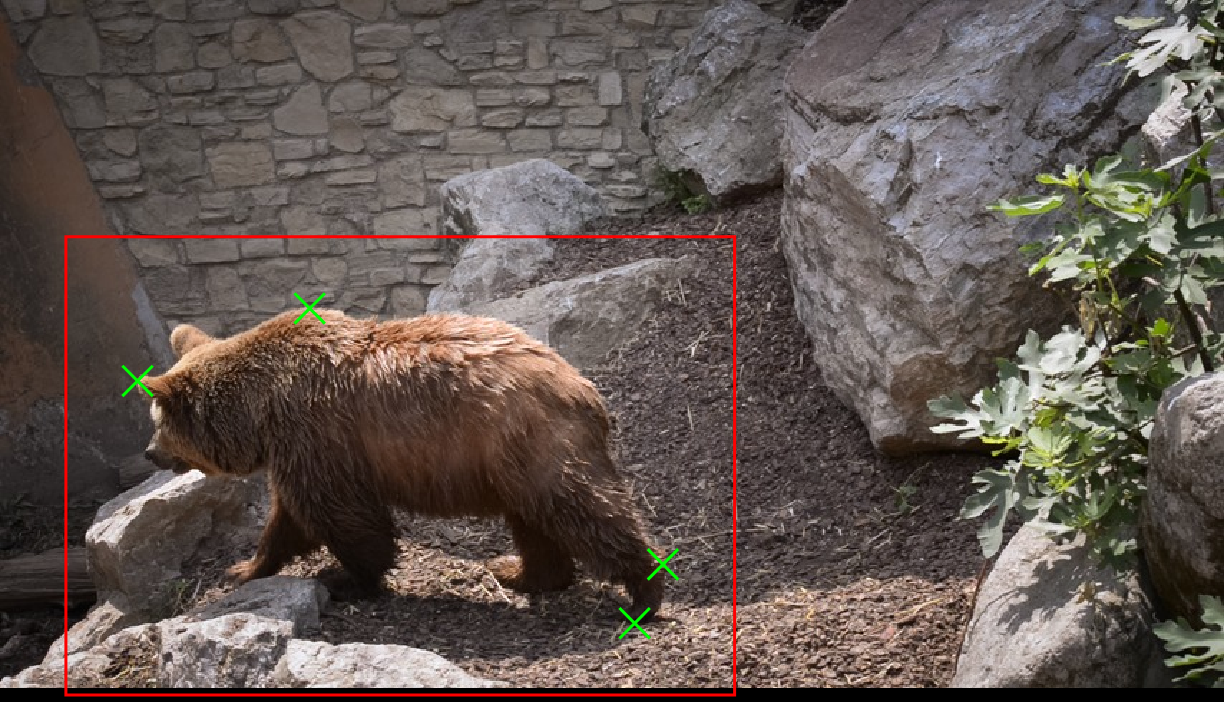
\includegraphics[width=\linewidth]{figures/chap33_bear_bbox.png}
	\caption[DEXTR User Interaction]{		
		Image with the obtained user input for the \gls{dextr} method and the first processing step.
		The extreme points are visualized as green crosses.
		The bounding box is enlarged by $p_{{box}} = 50$ \Unit{px}, shown in red.
		The enlarged bounding box extends the image boundary, therefore \textit{zero padding} is applied.
		The corresponding cropped and resized image is shown in Figure \ref{fig:ch3:sec3:rgb_channel}.
	}
	\label{fig:ch3:sec3:user_interaction}
\end{figure}


% One feature map with extreme points
Second, the four extreme points are converted into one heatmap.
The points in this heatmap are located on the boundary of the object.

To highlight the extreme points a 2D Gaussian is centered around each point $ \textbf{p} (x_p, y_p) $ with the another points $ \mathbf{x} = (x, y) $ by
% Impelemtation in HDevelop:
% ResGauss := exp(-4 \cdot log(2) $\cdot$ ((Rows-PointRow)*(Rows-PointRow) + (Cols-PointCol)*(Cols-PointCol)) / (GaussSigma * GaussSigma))
\begin{equation} \label{equ:gauss}
	\centering
	Gauss \left( x,y \right)  = max \left( g\left( x,y\right) , \frac{\exp(- 4 \log_{2}(| \textbf{x} - \textbf{p} |_2)}{\sigma^{2}}\right) 
\end{equation}
where $ g (x,y) $ is the current grayvalue of the heatmap at position $ (x, y) $ and $ \sigma = 10 $ representing the standard deviation of the Gauss filter.
This heatmap is vital for the method, because of the high level guidance for the deep segmentation network.
A closeup of a point centered by the 2D Gaussian is visualized in Figure \ref{fig:ch3:sec3:gauss_centered_point}.

Third, the heatmap has the size of $512 \times 512$ \Unit{px} and is concatenated with the RGB image.
This results in the four-channel \gls{dextr} model input, which is illustrated in Figure \ref{fig:ch3:sec3:model_input_channels}.

\begin{figure}
	\centering
	\begin{subfigure}[b]{0.3\textwidth}
		\centering
		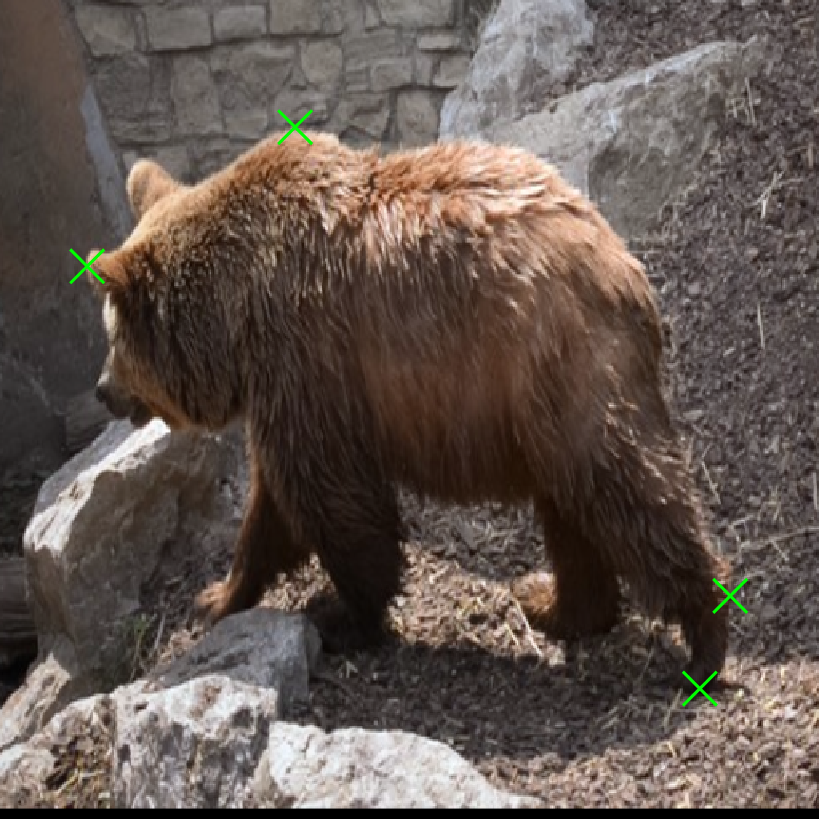
\includegraphics[width=\textwidth]{figures/chap33_channel_rgb.png}
		\caption{RGB image cropped based on the bounding box (three channels).}
		\label{fig:ch3:sec3:rgb_channel}
	\end{subfigure}
	\hfill
	\begin{subfigure}[b]{0.3\textwidth}
		\centering
		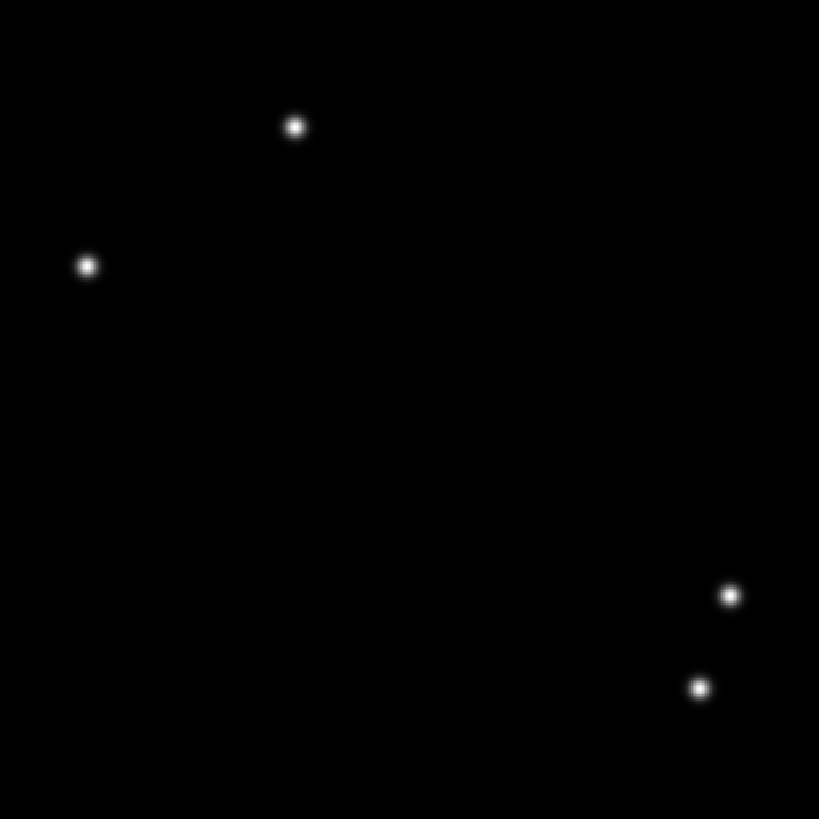
\includegraphics[width=\textwidth]{figures/chap33_channel_fg.png}
		\caption{Foreground heatmap with four extreme points (one channel).}
		\label{fig:ch3:sec3:fg_channel}
	\end{subfigure}
	\hfill
	\begin{subfigure}[b]{0.3\textwidth}
		\centering
		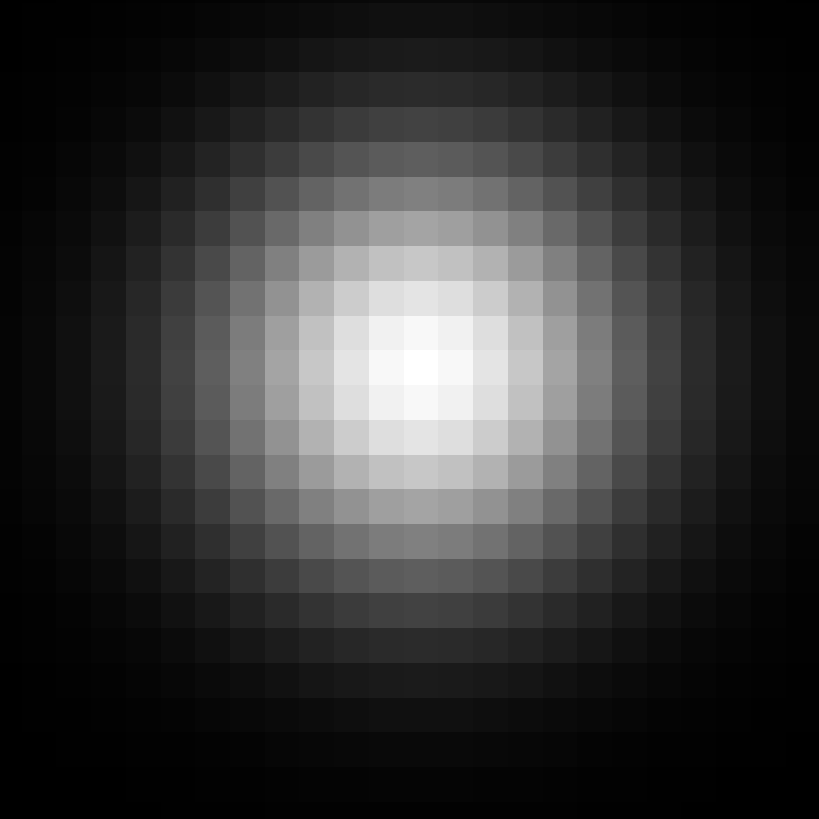
\includegraphics[width=\textwidth]{figures/chap33_gaussian_point.png}
		\caption{Closeup of a point centered with a 2D Gaussian with $\sigma = 10$.}
		\label{fig:ch3:sec3:gauss_centered_point}
	\end{subfigure}
	\caption[Four-channel DEXTR model input]{
		Representation of the separate channels from the four-channel \gls{dextr} model input.
		All channels have the spacial dimension of $512 \times 512$ \Unit{px}.
		The user points on the object's boundary are processed by the 2D Gaussian.
	} \label{fig:ch3:sec3:model_input_channels}
\end{figure}


\subsection{Architecture}\label{ord:ch3:sec3:subsec3}

As encoder for the segmentation network \textit{ResNet-101} \cite{He16-ResNet} is selected, which also referred to as \textit{backbone}.
The ResNet-101 is a deep \gls{cnn} containing 101 layers.
The core components of any ResNets are \textit{residual units}, whose main feature is the use of skip connections \cite{Ger17-HandsOn}.
The ResNet-101 is structured in four blocks, that contain 3, 4, 23 and 3 bottleneck blocks.

The ResNet-101 used for \gls{dextr} is modified by including atrous convolution in the last two blocks and removing the fully connected layers.
After the backbone a four staged \gls{psp} module is applied to preserve global context.
The decoder of this architecture does not consist of several convolution layers, instead bilinear interpolation is used to retrieve original spatial dimension of $512 \times 512$ \Unit{px}.
Finally, a sigmoid function is applied to obtain the final prediction $\textbf{y}$ as a  probability map. \footnote{Wolfram Math world, Sigmoid Function\url{https://mathworld.wolfram.com/SigmoidFunction.html}}

% Training settings.
The model is trained for $ n_{epochs} = 100 $ epochs on the PASCAL \gls{voc} 2012 Segmentation and further $ n_{epochs} = 10 $ epochs on the COCO dataset.
The learning rate is $ \lambda = 10^{-8} $ and the momentum is $ 0.9 $.


\subsection{Refinement}\label{ord:ch3:sec3:subsec4}

As introduced in Subsection \ref{ord:ch2:sec3:subsec2}, some interactive methods provide the possibility to perform refinement, if a segmentation result does not meet the user's expectations.
For the \gls{dextr} method the user may perform refinement by setting an additional click.
The refinement click should be located on the boundary of the region where the segmentation fails.
This new refinement click is added to the foreground heatmap with the extreme points.
In Figure \ref{fig:ch3:sec3:refinement} the effect of an additional refinement click is exemplary presented.
Each refinement click triggers a new model execution.
The refinement process may be applied iteratively.

% TODO plots use an example where the initial prediction actually fails and the refinement succeeds.
\begin{figure} 
	\centering
	\begin{subfigure}[b]{0.45\textwidth}
		\centering
		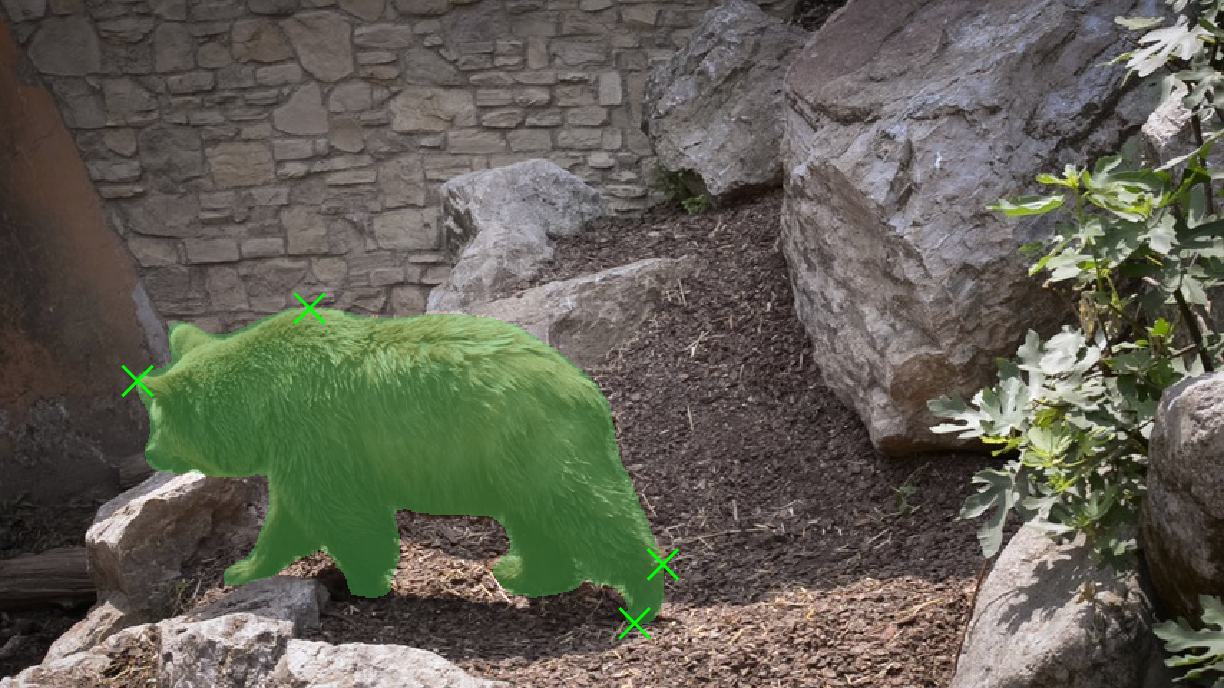
\includegraphics[width=\textwidth]{figures/chap33_bear_initial_result.png}
		\caption{Initial segmentation result.}
		\label{fig:ch3:sec3:refinement_1}
	\end{subfigure}
	\hfill
	\begin{subfigure}[b]{0.45\textwidth}
		\centering
		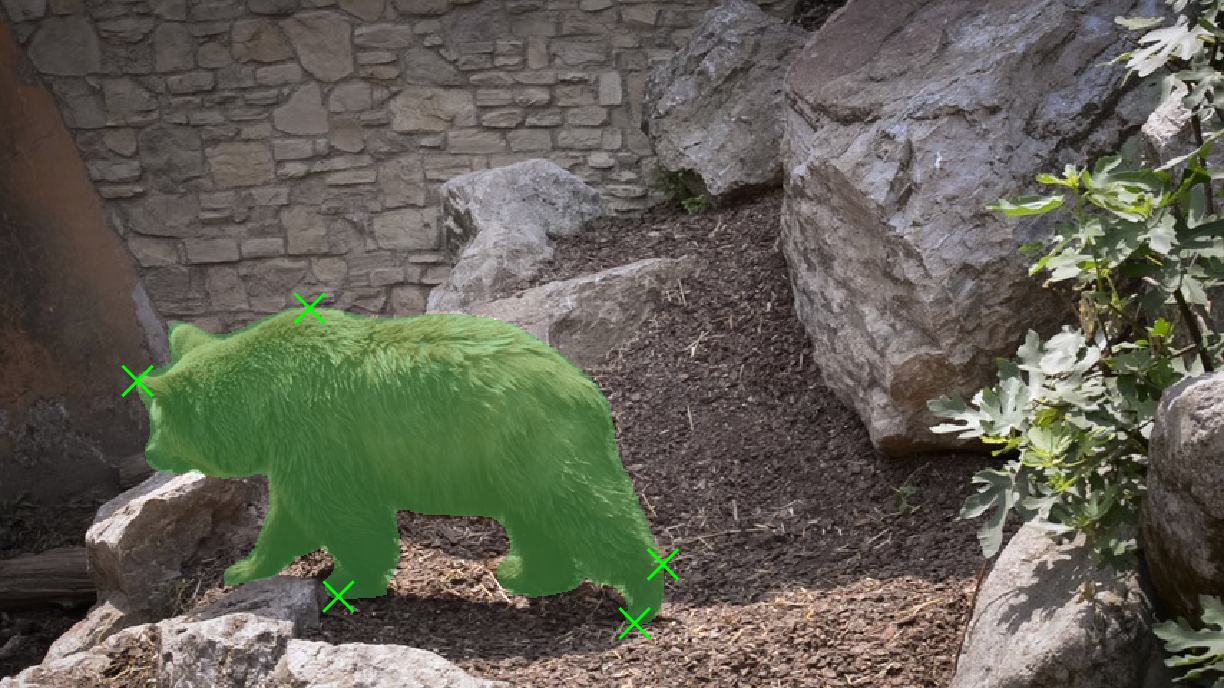
\includegraphics[width=\textwidth]{figures/chap33_bear_refine_result.png}
		\caption{Refinement segmentation result.}
		\label{fig:ch3:sec3:refinement_2}
	\end{subfigure}
	\caption[DEXTR Refinement]{
		On the left is the initial result with the normal extreme points. 
		On the right is the segmentation result with one additional refinement click.
	} \label{fig:ch3:sec3:refinement}
\end{figure}


\subsection{Performance}\label{ord:ch3:sec3:subsec5}

The performance of the \gls{dextr} method in comparison to other interactive segmentation methods in shown in Table \ref{tab:ch2:interactive-stae-of-the-art}.
In this comparison on PASCAL \gls{voc} the \gls{dextr} method performs well and is only outperformed by the \gls{iog} method.

The experiments and evaluations presented in \cite{Man18-DEXTR} contain various datasets and test settings.
Among them is also an examination of the performance on unseen classes and the generalization capability of the method.
Thereby, the model was trained with the PASCAL \gls{voc} or COCO dataset and evaluated on both datasets.
Despite these results seem reliable, it must be taken into account that the PASCAL \gls{voc} and COCO datasets are very similar and cover the same type of \textit{general} objects.
The evaluation of the generalization capabilities of the method continues in detail in Section \ref{ord:ch5:sec2_generalization_image_domains}.

An introduced application for the \gls{dextr} method is to create annotations and use them as new \gls{gt} to train \gls{dl} models.
Manisis \etal claim, that models trained on \gls{dextr} annotations perform equally well as models trained on the original \gls{gt}\cite{Man18-DEXTR}.
This statement is further examined in Section \ref{ord:ch5:sec5_retrain}.
% !TeX root = ../../main.tex
% Add the above to each chapter to make compiling the PDF easier in some editors.

\section{Inside-Outside Guidance}\label{ord:ch3:sec4}

Another approach for interactive segmentation is the \gls{iog} method, introduced in \cite{Zha20-IOG}.
The concept of this state-of-the-art method is strongly based on the previously introduced \gls{dextr} method \cite{Man18-DEXTR}.

\subsection{Basic Concept}\label{ord:ch3:sec4:subsec1}
% User Clicks - Workflow
The user interaction of the \gls{iog} method requires three user clicks executed in two steps.
First, the user has to draw a tight bounding box around the object of interest. 
The drawing of the bounding box may be counted as two user clicks on the background or one stroke.
% TODO refine the stroke possibility
%The creation of the bounding box is implemented using a stroke instead of setting two clicks.
Second, the user has to click once on the center of the object, which is represented as foreground click. 
The described workflow is illustrated in Figure \ref{fig:ch3:sec4:iog_user_clicks}.
Further, the user clicks are processed and an object mask is predicted by a \gls{dl} model.

% Naming of the method
% two-fold
The user provides high level guidance on the foreground and background, representative for the inside and outside region of the object.
On the one hand, this guidance is based on the bounding box that defines the background.
So, everything outside the bounding box does not belong to the object, this is described as \textit{outside} guidance.
On the other hand, the foreground click provides explicit guidance, where the object is located.
This is referred to as \textit{inside} guidance.
These two types of guidance are the namesake of the method \glsentryfull{iog}.
% TODO Auch wenn die Box-Ecken als "background" heatmap verwendet/bezeichnet wird glaube ich, dass das Modell auch lernt, dass sich das Objekt immer innerhalb der Eckpunkte befindet. Die Experimente von Matthias, als er auch mal erlaubt hatte, dass die Box das Objekt nicht ganz überdeckt sind ja glaube ich auch deutlich schlechter ausgefallen. Insofern bieten auch die Box-Eckpunkte eine Art "inside" guidance

% Advantage over DEXTR
Zhang \etal claim, that their way to set user clicks has two advantages compared to the way to set user clicks in other interactive methods as \gls{dextr}.
First, setting of extreme points may be confusing and misleading, as they may be located very close to each other, depending on the orientation of the object.
Second, if the object of interest contains a hole (\eg a donut) or is in the background of another object, \gls{dextr} cannot provide a robust guidance.
In contrast, the variable position of the foreground click in \gls{iog} enables a more robust guidance even for special object scenarios \cite{Zha20-IOG}.

\begin{figure}
	\centering
	\begin{subfigure}[b]{0.3\textwidth}
		\centering
		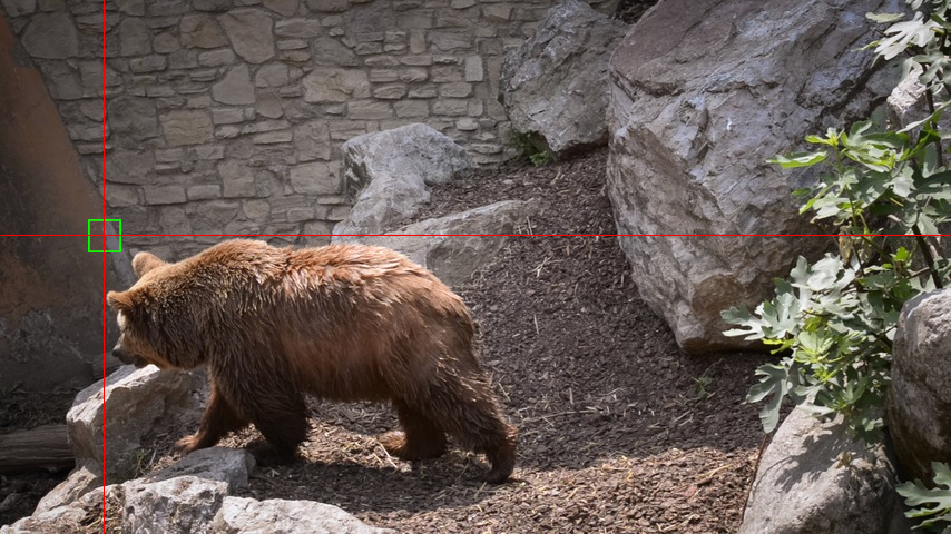
\includegraphics[width=\textwidth]{figures/chap34_bear_2.png}
		\caption{First background click.}
		\label{fig:ch3:sec4:iog_workflow_1}
	\end{subfigure}
	\hfill
	\begin{subfigure}[b]{0.3\textwidth}
		\centering
		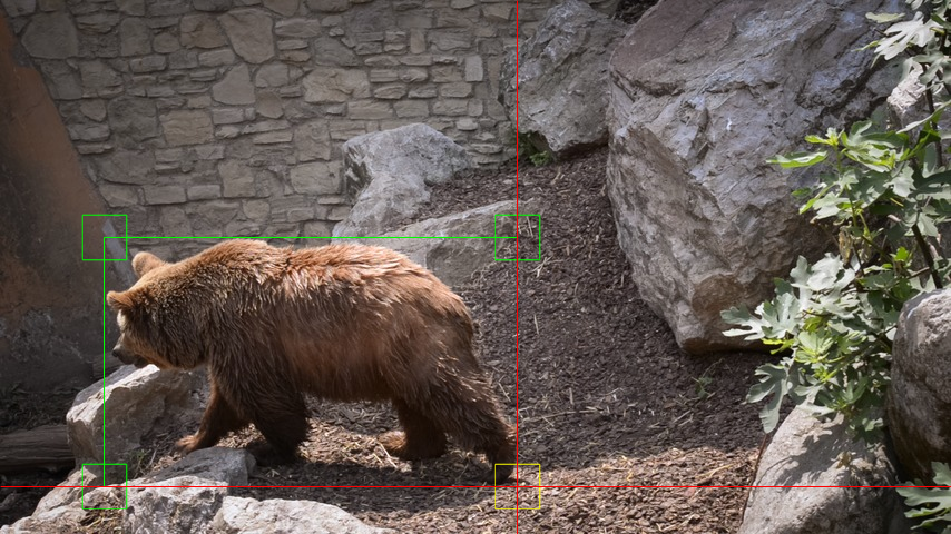
\includegraphics[width=\textwidth]{figures/chap34_bear_3.png}
		\caption{Second background click.}
		\label{fig:ch3:sec4:iog_workflow_2}
	\end{subfigure}
	\hfill
	\begin{subfigure}[b]{0.3\textwidth}
		\centering
		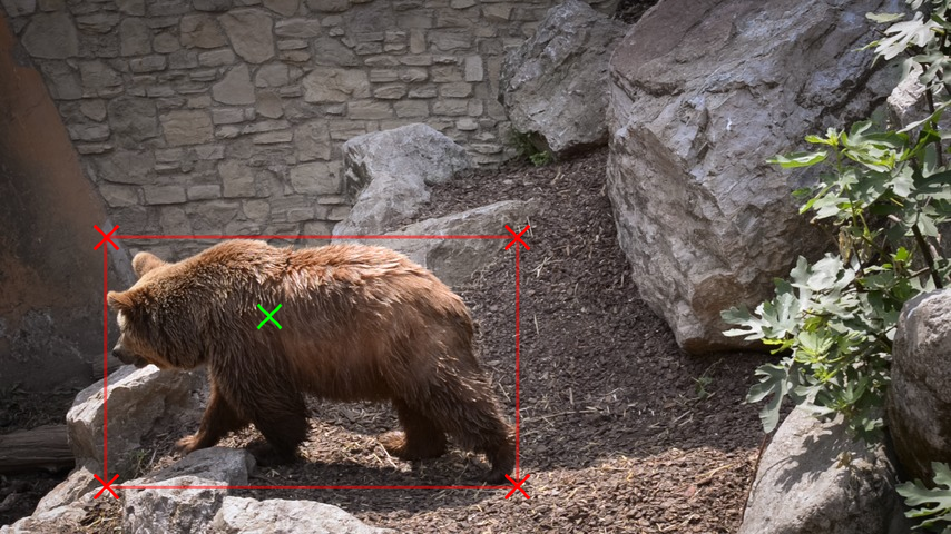
\includegraphics[width=\textwidth]{figures/chap34_bear_5.png}
		\caption{Foreground click.}
		\label{fig:ch3:sec4:iog_workflow_3}
	\end{subfigure}
	\caption[IOG User Interaction]{
		Shown is the workflow to perform the user interaction required for the \gls{iog} method.
		First, a bounding box is spanned by setting two background clicks.
		Last, the foreground click is set.
		All used points are visualized with a cross, background points in red and the foreground point in green, while the contour of the bounding box is drawn in red.
	} 
	\label{fig:ch3:sec4:iog_user_clicks}
\end{figure}

\subsection{Model Input and Representation of User Clicks}\label{ord:ch3:sec4:subsec2}

Identical to the \gls{dextr} method, the background clicks form a bounding box, which is enlarged by  $p_{{box}}$ \Unit{px}.
This processing is identical to the \gls{dextr} method.
% TODO ??mention that the background points are move by ~10 pixel in order to avoid the enforced background points being on the foreground
The image is cropped based on the enlarged bounding box and resized to the size of $512 \times 512$ \Unit{px}, if necessary zero padding is applied.

The bounding box is formed by the two background points, that are diagonal corners points (top-left and bottom-right or bottom-left and top-right).
Based on these two points, the other two corner points are derived, which provides four background points for the price of two.
As in the \gls{dextr} processing, the fore- and background clicks are converted into points on two separate heatmaps.
To highlight the user points a 2D Gaussian is centered around each click (see Equation \ref{equ:gauss}).

The two heatmaps have the size of $512 \times 512$ \Unit{px} and are concatenated with the \Gls{rgb} image.
This results in the five-channel \gls{iog} model input, which is explanatory illustrated in Figure \ref{fig:ch3:sec4:model_input_channels}.

%TODO add crosses to cropped RGB image
\begin{figure}
	\centering
	\begin{subfigure}[b]{0.3\textwidth}
		\centering
		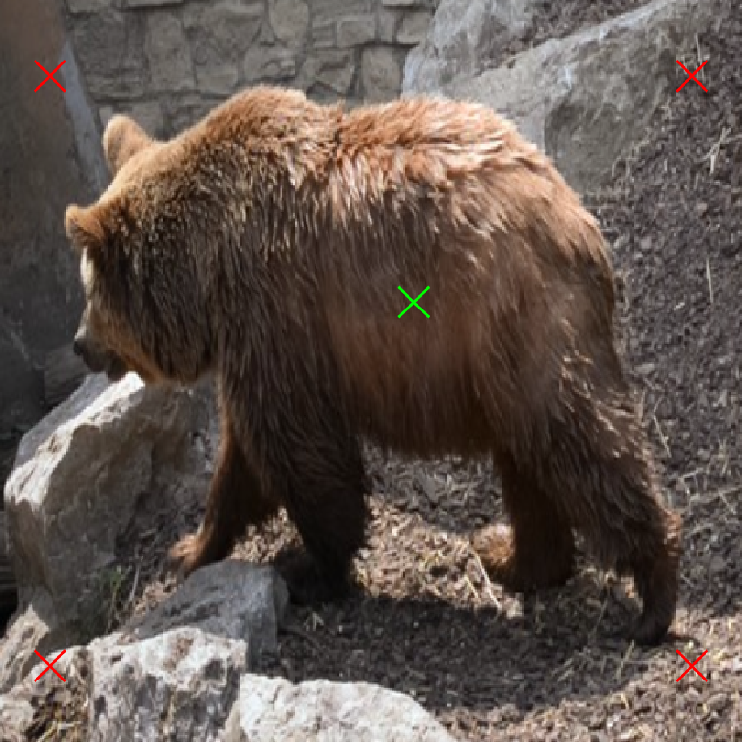
\includegraphics[width=\textwidth]{figures/chap34_channel_rgb.png}
		\caption{RGB image cropped based on the bounding box (three channels).}
		\label{fig:ch3:sec4:rgb_channel}
	\end{subfigure}
	\hfill
	\begin{subfigure}[b]{0.3\textwidth}
		\centering
		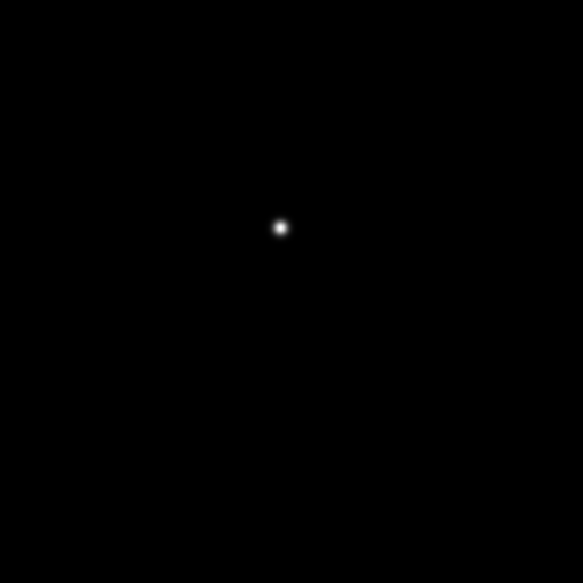
\includegraphics[width=\textwidth]{figures/chap34_channel_fg.png}
		\caption{Foreground heatmap with one foreground point (one channel).}
		\label{fig:ch3:sec4:fg_channel}
	\end{subfigure}
	\hfill
	\begin{subfigure}[b]{0.3\textwidth}
		\centering
		
\includegraphics[width=\textwidth]{figures/chap34_channel_bg.png}
		\caption{Background heatmap with four background points (one channel).}
		\label{fig:ch3:sec4:bg_channel}
	\end{subfigure}
	\caption[Five-channel IOG model input]{
		Representation of the separate channels from the five-channel \gls{iog} model input.
		All channels have the spatial dimension of $512 \times 512$ \Unit{px}.
		The user points in the foreground and background heatmaps are enforced with a 2D Gaussian.
	} \label{fig:ch3:sec4:model_input_channels}
\end{figure}

\subsection{Architecture}\label{ord:ch3:sec4:subsec3}

The model architecture used for the \gls{iog} method is based on the encoder-decoder architecture and special structure for layer fusion.
The encoder-decoder network is titled as \textit{CoraseNet}, while the structure for layer fusion is referred to as \textit{FineNet}.
An illustration of the complete architecture is given in Figure \ref{fig:ch3:sec4:arch}.


\subsubsection{CoarseNet}
The CoarseNet consists out of multiple components: encoder network, decoder network, \gls{psp}-module and skip connections. The CoarseNet is built upon the \gls{dextr} method, therefore they partially share the same architectural components.

As in the \gls{dextr} architecture, the encoder network is represented by ResNet-101 \cite{He16-ResNet}, followed by a \gls{psp} module.
%The ResNet is implemented without the head of fully connected layers. It contains four ResNet blocks and the fourth block outputs 2048 feature maps of the size $32 \times 32$ \Unit{px}.
% As in \gls{dextr} a \gls{psp}-module is applied after the backbone to gain more contextual information.
The output of the \gls{psp}-module is a coarse prediction with the spatial dimension of  $32 \times 32$ \Unit{px} containing 512 feature maps. 

From this onward the decoder network starts the upsampling process.
% TODO declare what kind of operations are used for the upsampling.
The decoder network is built upon a reversed, simplified version of the encoder architecture. % , that consists out of four residual blocks.
Therefore, the decoder network is based on four blocks, in order to regain the original input size of  $512 \times 512$ \Unit{px}.
Further, three skip connection are applied and establish a connection in between the four resiudual blocks of the encoder and decoder network, as visualized in Figure \ref{fig:ch3:sec4:arch}.
% TODO this skip connection also does some processing
% During the upsampling process activations from the residual blocks of the ResNet are transferred from the ResNet using so lateral connections and concatenated with the upsampled feature maps.
% A benefit of this architecture is the fusion of information from different network stages.
\begin{figure}
	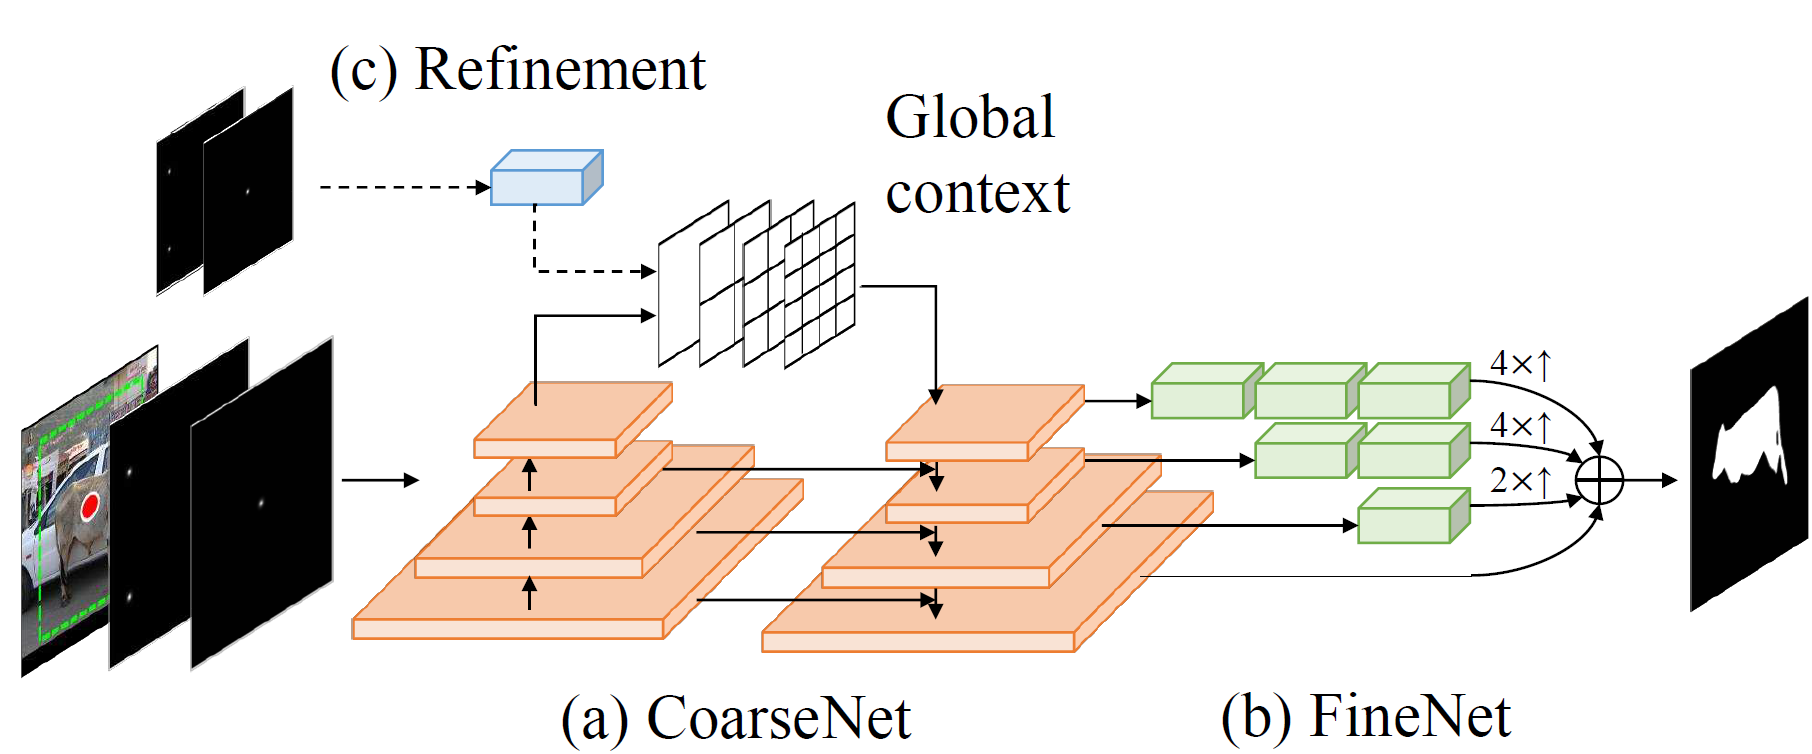
\includegraphics[width=\linewidth]{figures/chap34_iog_arch.png}
	\caption[IOG Architecture]{		
		Architecture of the \gls{iog} model.
		On the left the model input is visualized as in Figure \ref{fig:ch3:sec4:model_input_channels}.
		The CoarseNet is marked by (a) and shows the encoder and decoder network with the skip connections and the \gls{psp} module.
		The FineNet is marked by (b) and represents the four stream fusion structure.
		It can be seen, that the single streams origin from different levels of the decoder network.
		In order to obtain a common spatial dimension for concatenation $ \oplus $, the streams differ in their processing.
		As final prediction a binary object mask is shown.
		The lightweight-branch for refinement is marked with (c).
		Copyright \copyright 2020 IEEE. Reprinted by permission from \cite{Zha20-IOG}.
	}
	\label{fig:ch3:sec4:arch}
\end{figure}

\subsubsection{FineNet}
The FineNet consists of a four-stream fusion structure.
The four streams originate from the four levels of the decoder network and, therefore, process feature maps of various sizes (see Figure \ref{fig:ch3:sec4:arch}).
Each stream processes and upsamples the feature maps by a descending number of bottleneck processing blocks.
The streams reconstruct the feature maps to the final spatial dimension of $512 \times 512$ \Unit{px}.
%applied in order to use \emph{"features at deeper layers for better trade-off between accuracy and efficiency"} \cite[p. 12237]{Zha20-IOG}.
In the end the four streams are concatenated and pass through a final bottleneck processing block.
To the final output a sigmoid is applied, which results in a probability map as final prediction of the \gls{iog} network.

The author justifies the application of these different components by showing their effect in an ablation study \cite{Zha20-IOG}.
% The author shows in an ablation study, that the FineNet enhances the networks IoU by $0.8\%$. 
% The ablation study is performed with a ResNet-50 as backbone and PASCAL-1k \cite{Eve20-PascalVOC} as dataset. 


\subsection{Refinement}\label{ord:ch3:sec4:subsec4}

To perform refinement in the \gls{iog} method, the user sets an additional click on the largest fore- or background region that was predicted wrongly.
Identically to the \gls{dextr} method, refinement may be performed iteratively and each refinement click triggers a model execution.
However, in contrast to \gls{dextr} the refinement of the \gls{iog} method does not require the execution of the complete model, but just the refinement part the FineNet.

The integration in the existing architecture is realized as follows.
New heatmaps for fore- and background are created with the original clicks and the refinement clicks.
These two heatmaps are combined into a two-channel input, which is processed in a so called lightweight-branch.
This lightweight-branch consists out of five convolutional layers, that perform the downsampling.
The output of this branch is combined with the output of the initial iteration from the encoder network and forwarded to the \gls{psp} module as shown in Figure \ref{fig:ch3:sec4:arch}.
This means that the computationally expensive encoder must only be executed for the initial prediction.
From the \gls{psp} module onwards the model is executed normally.

Hence, the encoder network does not require a new execution and the execution of the model time is decreased.
Zhang \etal state, that the usage of the lightweight-branch performs better than directly adding the refinement click into the normal five-channel input.

% TODO use an example where the initial prediction actually fails and the refinement succeeds.
\begin{figure} 
	\centering
	\begin{subfigure}[b]{0.45\textwidth}
		\centering
		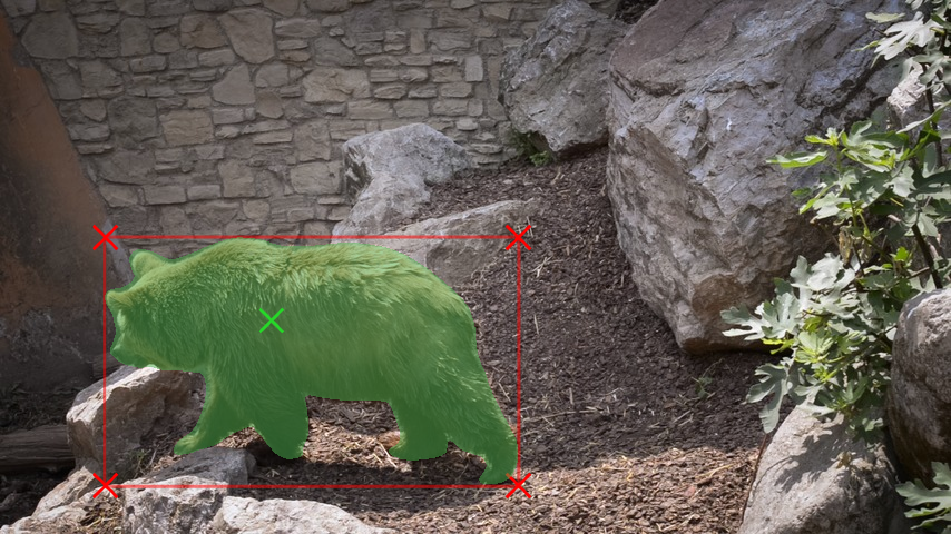
\includegraphics[width=\textwidth]{figures/chap34_bear_6.png}
		\caption{Initial segmentation result.}
		\label{fig:ch3:sec4:refinement_1}
	\end{subfigure}
	\hfill
	\begin{subfigure}[b]{0.45\textwidth}
		\centering
		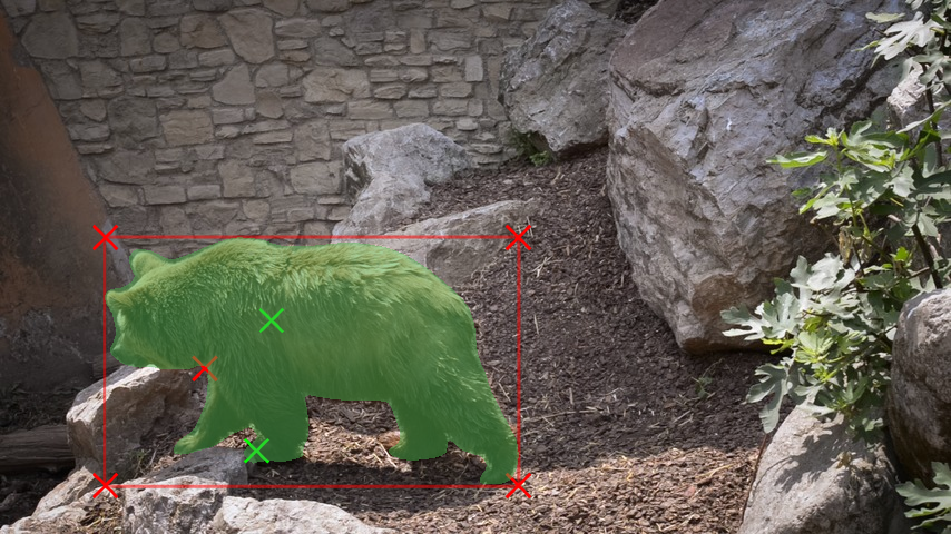
\includegraphics[width=\textwidth]{figures/chap34_bear_8.png}
		\caption{Refinement segmentation result.}
		\label{fig:ch3:sec4:refinement_2}
	\end{subfigure}
	\caption[IOG Refinement]{
		On the left is the initial result with the normal amount of clicks. 
		On the right is the results of two refinement iterations with one additional refinement click on the foreground and one on the background.
	} \label{fig:ch3:sec4:refinement}
\end{figure}


\subsection{Performance}\label{ord:ch3:sec4:subsec5}

An overview of interactive segmentation methods is presented in Table \ref{tab:ch2:interactive-stae-of-the-art}.
It can be seen that the \gls{iog} outperforms other state-of-the-art methods with respect to the number of set points to reach a certain IoU-level and the achieved \gls{iou} at exactly four clicks.

% TODO Comment von Paddo - Ist das etwas was du rausgefunden hast oder steht das so im Paper oder ist das deine Intuition? 
This method especially performs well due the highly connected architecture.
The application of skip connections and the FineNet enable the model to recover local details and prevent the information loss during down- and upsampling process.

Similar to the experiments performed in \cite{Man18-DEXTR}, Zhang \etal also investigate the performance on unseen classes and the generalization capability of the method \Cite{Zha20-IOG}. 
This topic will be continued by the evaluation of other unseen domains in Section \ref{ord:ch5:sec2_generalization_domains}.

Zhang \etal also evaluate the performance on dataset with other domains than PASCAL \gls{voc} (\eg Rooftops, CityScapes, or Agricultural-Vision).
Further, it is demonstated in various setups, that the \gls{iog} method trained on PASCAL \gls{voc} outperformed the \gls{dextr} method or the \textit{Curve-\gls{gcn}}, both trained on the CityScapes dataset.

% TODO appendix with various examples of IOG segmentation results?